\subsection{Overview}


UrbanSim has been developed to support land use, transportation and environmental planning, with particular attention to the regional transportation planning process \citep{waddell-japa-2002, waddell-tra-2007, waddell-tr-2011}. It has been designed to perform several tasks.

%\todo{From Emily regarding land use footnote: I would delete the part of the footnote that says "not only to the use of land" - this is pretty clear.}

\begin{enumerate}
\item It can predict land use\footnote{We use the term \emph{land use} broadly, to represent the characteristics of real estate development and prices, and the location and types of households and businesses.} information for input to the travel model, for periods of 10 to 40 years into the future, as needed for regional transportation planning.

\item It can predict the effects on land use patterns from alternative investments in roads and transit infrastructure, alternative transit levels of service, or alternative roadway and transit pricing, over long-term forecasting horizons. Scenarios can be compared using different transportation network assumptions to evaluate the relative effects on development from a single project or a more wide-reaching change in the transportation system, such as extensive congestion pricing.

\item It can predict the effects of changes in land use regulations on land use. This includes the effects of policies to relax or increase regulatory constraints on development of different types, such as an increase in the allowed Floor Area Ratios (FAR) on specific sites, or allowing mixed-use development in an area previously zoned only for one use.

\item It can predict land use development patterns induced by investments in transit.

\item It can predict the effects of environmental policies that impose constraints on development, such as protection of wetlands, floodplains, riparian buffers, steep slopes, or seismically unstable areas.

\item It can predict the effects of changes in the macroeconomic structure or growth rates on land use. Periods of rapid or slow growth, or even decline in some sectors, can lead to changes in the spatial structure of the city and the model system is designed to analyze these shifts.

\item It can predict the possible effects of changes in demographic structure and composition of the city on land use and on the spatial patterns of clustering of residents of different social characteristics, such as age, household size, and income.

\item It can examine the potential impacts of major development projects (both actual and hypothetical) on land use and transportation. This can be used to explore the impacts of a corporate relocation or to compare alternative sites for a major development project.
\end{enumerate}

% UrbanSim was designed to reflect the interdependencies in dynamic urban systems with an initial focus on the real estate market and the transportation network. UrbanSim can also be used to consider the effects of individual interventions and combinations of interventions on patterns of development, travel demand, and household and firm location. Some goals that have shaped the design of UrbanSim, and some that have emerged through the past several years real world testing include:

% \begin{itemize}

%     \item Enable a wide variety of stakeholders (planners, public agencies, citizens, and advocacy groups) to explore the potential consequences of alternative public policies and investments using credible, unbiased analysis.
    
%     \item Facilitate more effective democratic deliberation on contentious public actions regarding land use, housing, transportation, and the environment informed by the potential consequences of alternative courses of action that include long-term cumulative effects on the environment and distributional equity considerations.
    
%     \item Make it easier for communities to achieve a common vision for the future of the community and its broader environment and to coordinate their actions to produce outcomes that are consistent with this vision.
    
%     \item Create an analytical capacity to model the cause and effect interactions within local urban systems that are sufficiently accurate and sensitive to policy interventions to be a credible source for informing deliberations.
    
%     \item Make the model system credible by avoiding bias in the models through simplifying assumptions that obscure or omit important cause-effect linkages at a level of detail needed to address stakeholder concerns. Note that this is particularly relevant for housing policies: most urban models do not directly represent rental and ownership components of the housing market separately and none other than UrbanSim work at a microsimulation level representing individual persons, households, parcels, buildings, and even housing units within buildings.
    
%     \item Make the model design behaviorally clear in terms of representing agents, actions, and cause--effect interactions in ways that can be understood by non-technical stakeholders, while making the statistical methods used to implement the model scientifically robust.
    
%     \item Make the model system open, accessible, and transparent by adopting an Open Source licensing approach and releasing the code and documentation on the web.
    
%     \item Encourage the development of a collaborative approach to development and extension of the system through open source licensing and web access and by design choices and supporting organizational activities.
    
%     \item Test the system extensively and repeatedly and continually improve it by incorporating lessons learned from applications and from new advances in methods for modeling, statistical analysis, and software development.
    
% \end{itemize}

% The original design of UrbanSim adopted several elements to address these implementation goals, and these have remained foundational in the development of the system over time. These design elements include:

% \todo{From Emily: In the second item below does "fine" mean granular? If yes, we should use the word "granular"}

% \begin{itemize}

%     \item The representation of individual agents: initially households and firms, and later persons and jobs.
    
%     \item The representation of the supply and characteristics of land and of real estate development at a fine spatial scale depending on the needs of the user and availability of data: from parcels and buildings to census blocks or user-defined zones.
    
%     \item The adoption of time dynamics, with the simulation proceeding in annual steps and the urban system evolving in a path dependent manner.
    
%     \item The use of real estate markets as a central organizing focus with consumer choices and supplier choices explicitly represented as well as the resulting effects on real estate prices. The relationship of agents to real estate tied to specific locations providing a clean accounting of space and its use.
    
%     \item The use of standard discrete choice models to represent the choices made by households and firms and developers (principally location choices). To date, this has relied principally on the traditional Multinomial Logit (MNL) specification.
    
%     \item Integration of the urban simulation system with existing transportation model systems to obtain information used to compute accessibilities and their influence on location choices and to provide raw inputs to the travel models.
    
%     \item The adoption of an Open Source licensing for the software, written originally in Java, and recently reimplemented using the Python language with extensive use of numerical libraries implemented in C or C++ for enhanced computational performance.

% \end{itemize}

% The key features of the UrbanSim model and its software implementation are highlighted in Table \ref{tab:key-features}. The model departs from prior operational land use models based on cross-sectional, equilibrium, aggregate approaches to adopt an approach that models individual households, jobs, buildings and parcels (or census blocks or zones), and their changes from one year to the next as a consequence of economic changes, policy interventions, and market interactions.

% \todo{From Emily: The preceding sentence starting with "The model departs from prior operational.." is too long - consider shortening}

% \todo{From Emily: The table below is mostly a bulleted list so not sure the table format is the best to use - maybe just used a bulleted list instead? Also in first bullet "development choices of developers" sounds weird to me}

% \begin{table}[htbp]
% \caption{Key features of UrbanSim}
% \label{tab:key-features}
% \begin{center}
% \begin{tabular}{ p{0.2\textwidth} p{0.7\textwidth} }
%     \toprule
    
%     \multirow[c]{10}{0.2\textwidth}{Key features of the UrbanSim model system}
%     & $\bullet$ Simulates the key decision makers and choices impacting urban development; in particular the mobility and location choices of households and businesses and the development choices of developers\\
%     & $\bullet$ Explicitly accounts for land, structures (houses and commercial buildings), and occupants (households and businesses)\\
%     & $\bullet$ Simulates urban development as a dynamic process over time and space, as opposed to a cross-sectional or equilibrium approach\\
%     & $\bullet$ Simulates the land market as the interaction of demand (locational preferences of businesses and households) and supply (existing vacant space, new construction, and redevelopment), with prices and rents adjusting to clear market\\
%     & $\bullet$ Housing markets are separated by tenure (owner and rental) as well as building type to represent the key differences on housing affordability and the impacts of increases in property values on the occupants of housing\\
%     & $\bullet$ Models housing supply decisions at the parcel level using development feasibility analysis (pro forma models) to evaluate the return on investment of a development project, considering its hard and soft costs as well as expected revenues from sale or from a stream of rents, discounted to the present\\
%     & $\bullet$ Incorporates governmental policy assumptions explicitly and evaluates policy impacts by modeling market responses\\
%     & $\bullet$ Based on random utility theory and uses logit models for the implementation of key demand components\\
%     & $\bullet$ Designed for high levels of spatial and activity disaggregation with a zonal system identical to travel model zones\\
%     & $\bullet$ Presently addresses both new development and redevelopment using parcel-level detail\\
    
%     \midrule
    
%     \multirow[c]{3}{0.2\textwidth}{Key features of the UrbanSim software implementation}
%     & $\bullet$ The model system runs on the cloud and uses a web browser for the User Interface\\
%     & $\bullet$ The UrbanSim model system software is open source\footnote{The open-source UrbanSim code base is available at \url{https://github.com/UDST/urbansim}}\\
%     & $\bullet$ The user interface focuses on creating, running and evaluating policy scenarios\\
    
%     \bottomrule
% \end{tabular}
% \end{center}
% \end{table}

% \subsection{Intended uses of the model system}

% UrbanSim has been developed to support land use, transportation and environmental planning, with particular attention to the regional transportation planning process. UrbanSim has been designed to perform several tasks.

% \todo{From Emily regarding land use footnote: I would delete the part of the footnote that says "not only to the use of land" - this is pretty clear.}

% First, UrbanSim can predict land use\footnote{We use the term \emph{land use} broadly, to refer not only to the
% use of land, but also to represent the characteristics of real estate development and prices, and the location and types of households and businesses.} information for input to the travel model, for periods of 10 to 40 years into the future, as needed for regional transportation planning.

% Second, UrbanSim can predict the effects on land use patterns from alternative investments in roads and transit infrastructure, alternative transit levels of service, or alternative roadway and transit pricing, over long-term forecasting horizons. Scenarios can be compared using different transportation network assumptions to evaluate the relative effects on development from a single project or a more wide-reaching change in the transportation system, such as extensive congestion pricing.

% Third, UrbanSim can predict the effects of changes in land use regulations on land use. This includes the effects of policies to relax or increase regulatory constraints on development of different types, such as an increase in the allowed Floor Area Ratios (FAR) on specific sites, or allowing mixed-use development in an area previously zoned only for one use.

% Fourth, UrbanSim can predict land use development patterns in high-capacity transit corridors.

% Fifth, UrbanSim can predict the effects of environmental policies that impose constraints on development, such as protection of wetlands, floodplains, riparian buffers, steep slopes, or seismically unstable areas.

% Sixth, UrbanSim can predict the effects of changes in the macroeconomic structure or growth rates on land use. Periods of rapid or slow growth, or even decline in some sectors, can lead to changes in the spatial structure of the city and the model system is designed to analyze these shifts.

% Seventh, UrbanSim can predict the possible effects of changes in demographic structure and composition of the city on land use and on the spatial patterns of clustering of residents of different social characteristics, such as age, household size, and income.

% Eighth and finally, UrbanSim can examine the potential impacts of major development projects (both actual and hypothetical) on land use and transportation. This can be used to explore the impacts of a corporate relocation or to compare alternative sites for a major development project.


% \subsection{Assumptions and limitations of the model system}

% UrbanSim is a model system and therefore an abstraction of reality. Only a small subset of the real world is reflected in the model system, as needed to address the kinds of uses outlined above. Like any model, or analytical method, that attempts to examine the potential effects of an action on one or more outcomes, there are limitations. Some important assumptions and limitations are discussed in the following subsections.

% \subsubsection{Boundary effects are ignored}
% \todo{From Emily: Is it weird to have a section header for a single sentence?}
% Interactions with adjacent metropolitan areas pose
% modeling difficulties due to boundary effects.

% \subsubsection{The land use regulations are assumed to be binding constraints on the actions of developers}

% This is equivalent to assuming that developers who wish to construct a project that is inconsistent with current land use regulations cannot get a waiver or modification of the regulations in order to accommodate the project. This assumption is more reflective of reality in some places than others, depending on how rigorously enforced land policies are in that location.

% There are cities in which developer requests for a variance from existing policies are met with little or no resistance. For UrbanSim, the limitation that it does not completely realistically simulate the way developers influence changes in local land use policies may be the most appropriate. It allows examination of the effects of policies, under the expectation that they are enforced, which allows more straightforward comparisons of policies to be made.

% \subsubsection{Large scale and microscopic events cannot be accurately predicted}

% The microscopic level of detail of UrbanSim can lead to the temptation to over-invest confidence in the micro-level predictions. Though the model as implemented in the Bay Area predicts the location choices of individual jobs, households, and developers, the intent of the model is to predict patterns rather than discrete individual events.

% No individual prediction made by the model, such as the development of a specific development project on a single parcel in 20 years from now, is likely to be correct. The tendencies for parcels in that area to have patterns or tendencies for development is what the model is intended to represent. Model users should therefore not expect to accurately predict large-scale, idiosyncratic events such as the development of a specific high-rise office building on a specific parcel. It would be advisable to aggregate results, and/or to generate multiple runs to provide a distribution of results.

% A related implication is that the lower level of sensitivity and appropriate use of the model system needs to be determined by a combination of sensitivity testing, experience from use, and common sense. It would not be likely, for example, that changing traffic signalization on a particular collector street intersection would be a large enough event to cause significant changes in model results.

% \subsubsection{Errors in input data will limit the model}

% Efforts were made to find obvious errors in the data, and to prevent these from affecting the results, but there was not sufficient time or resources to thoroughly address all data problems encountered, including some extreme values, missing values, and inconsistencies within and among data sources. The noise in the input data limits to some extent the accuracy of the model, though the statistical estimation of the parameters should help considerably in developing unbiased parameters even in the presence of missing data and other data errors.

% Over a long period of time, it would be worth investigating how much errors in input data change model results, and to fine-tune a strategy to invest in data where it makes the most effective use of scarce resources.

% \subsubsection{Behavioral patterns are assumed to be relatively stable over time}

% One of the most common assumptions in models, and one rarely acknowledged, is that behavioral patterns will not change dramatically over time. Models are estimated using observed data, and the parameters reflect a certain range of conditions observed in the data. If conditions were to change dramatically, such as fuel prices tripling, it is probable that fundamental changes in consumption behavior, such as vehicle ownership and use, would result.

\subsection{Inputs}

UrbanSim requires detailed representation of the built environment and its occupants.  It uses a microsimulation data structure, meaning that it represents every household, person, job, parcel, and building in a metropolitan area. The population data is generated from census data using synthetic population algorithms we have developed \citep{ye-trb-2009}.  The employment data is from an inventory of business establishments from the Metropolitan Transportation Commission, as is the parcel and building data for the 9 county San Francisco Bay Area. In addition, land use regulations from over 100 municipalities in the Bay Area were assembled and reconciled into a regional land use regulation database, and a database of development projects 'in the pipeline' for development was also assembled, to be able to accurately reflect development that is in progress.  Real estate prices and rents were obtained from CoStar for use in estimating the rent and price models in UrbanSim.  Finally, the California Household Travel Survey was used in estimating the Household Location Choice Model in UrbanSim.

In addition to the base data, the other main input to UrbanSim is what we refer to as scenario inputs. We use the term scenario in the context of UrbanSim in a very specific way: a scenario is a combination of input data and assumptions to the model system, including macroeconomic assumptions regarding the growth of population and employment in the study area, the configuration of the transportation system assumed to be in place in specific future years, and general plans of local jurisdictions that will regulate the types of development allowed at each location.

In order to facilitate comparative analysis, a model user such as a Metropolitan Planning Organization will generally adopt a specific scenario as a base of comparison for all other scenarios. This base scenario is generally referred to as the \enquote{baseline} scenario, and this is usually based on the adopted or most likely to be adopted regional transportation plan, accompanied by the most likely assumptions regarding economic growth and land use policies. Once a scenario is created, it determines several inputs to UrbanSim:

\begin{itemize}
    \item \textit{Control totals}: data on the aggregate amount of population and employment, by type, to be assumed for the region.
    \item \textit{Travel data}: data on zone to zone travel characteristics, from the travel model.
    \item \textit{Land use plan}: data on general plans, assigned to individual parcels.
    \item \textit{Development constraints}: a set of rules that interpret the general plan codes, to indicate the allowed land use types and density ranges on each parcel.
\end{itemize}

\subsection{How it works and what it does}

\subsubsection{The Role of Accessibility}

Accessibility is a well explored area of urban theory, and is the concept that connects transportation and land use, so is is central to understanding the UrbanSim model system.  Kevin Lynch in \textit{Good City Form} states, ``activities are assumed to locate according to the relative cost of reaching materials, customers, services, jobs, or labor.  Other values are simply subsidiary constraints in this struggle for access" \citep{lynch_good_1984}.  Lynch traces the original concepts to Wingo and Alonso \citep{wingo_transportation_1961,alonso_location_1964}, but the first explicit discussion is provided by Hansen \citep{hansen_how_1959}.

Operationally used accessibility frameworks include gravity-model based (defined by attractions and discounted by distance), cumulative-opportunity (summations within a set impedance measure) and space-time (limited by the opportunity prism of an individual's activity skeleton) \citep{kwan_space-time_1998,miller_measuring_1999}.  Dong and others expand on the space-time prisms by creating a logsum-based measure within a travel model \citep{dong_moving_2006}.  

To measure access, one must first choose a basic unit of geography to use.  The majority of transportation models in use today still rely heavily on zone-based geography for its simplicity and computational tractability \citep{hunt_current_2005}.  Zones can vary in size, but are usually a few city blocks at their smallest.  Drawbacks to this method include: the zones must be defined manually, they are arbitrary in scope, and they are too large to model micro-land use measures and walkability (which often vary on a block-by-block basis). We have developed algorithms to support walking scale queries on local street networks that enable fast accessibility queries to be computed on metropolitan scale networks \citep{foti2012generalized}.  In subsequent work we have generalized these algorithms to address walking plus transit networks \citep{blanchard2017urbanaccess, blanchard-waddell-trr-2017}. 


\subsubsection{Model system design and geographic level of analysis}

UrbanSim has been adapted to use at differing levels of geography. In this project, we use a parcel-level specification of the data and models in UrbanSim to support the maximum level of geographic detail, to avoid imposing aggregation bias on the model system. 


\begin{figure}[htbp]
    \center
    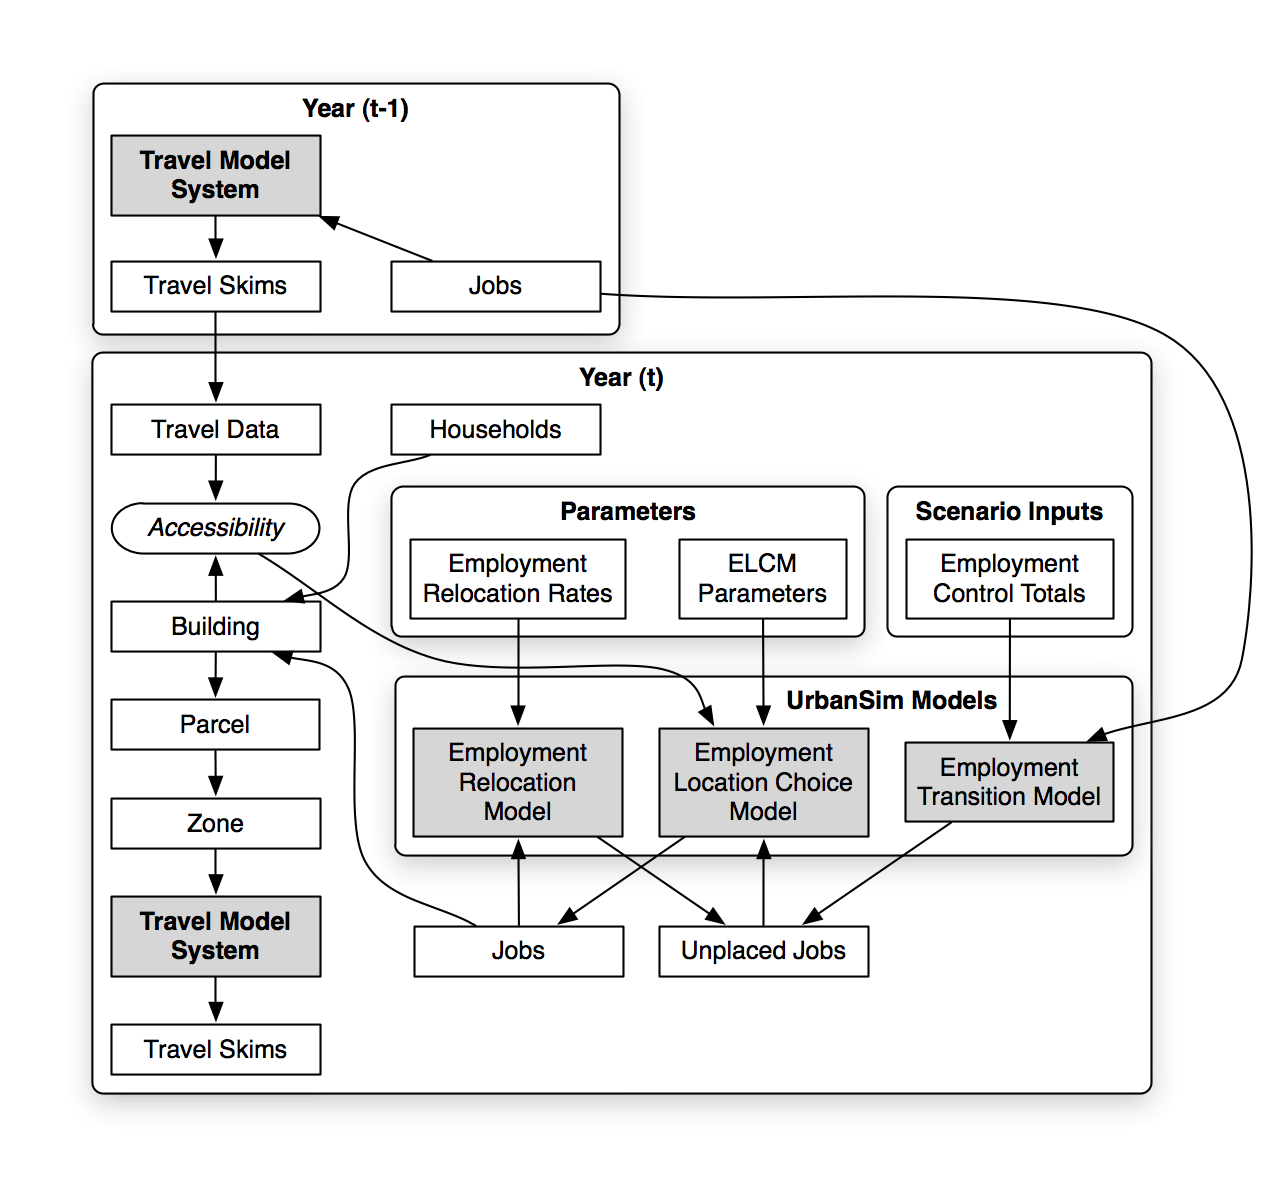
\includegraphics[width=\textwidth]{graphics/ParcelEmploymentModel.png}
    \caption{UrbanSim model flow: employment focus}
    \label{fig:employment-models}
\end{figure}

The components of UrbanSim are models acting on the objects in Figures \ref{fig:employment-models}, \ref{fig:household-models}, and \ref{fig:parcel-models}, simulating the real-world actions of agents in the urban system. Developers construct new buildings or redevelop existing ones. Buildings are located on land parcels that have particular characteristics such as value, land use, slope, and other environmental characteristics. Governments set policies that regulate the use of land, through the imposition of land use plans, urban growth boundaries, environmental regulations, and through pricing policies such as development impact fees. Governments also build infrastructure, including transportation infrastructure, which interacts with the distribution of activities to generate patterns of accessibility at different locations that in turn influence the attractiveness of these sites for different consumers. Households have particular characteristics that may influence their preferences and demands for housing of different types at various locations. Businesses also have preferences that vary by industry and size of business (number of employees) for alternative building types and locations.

\begin{figure}[ht]
    \center
    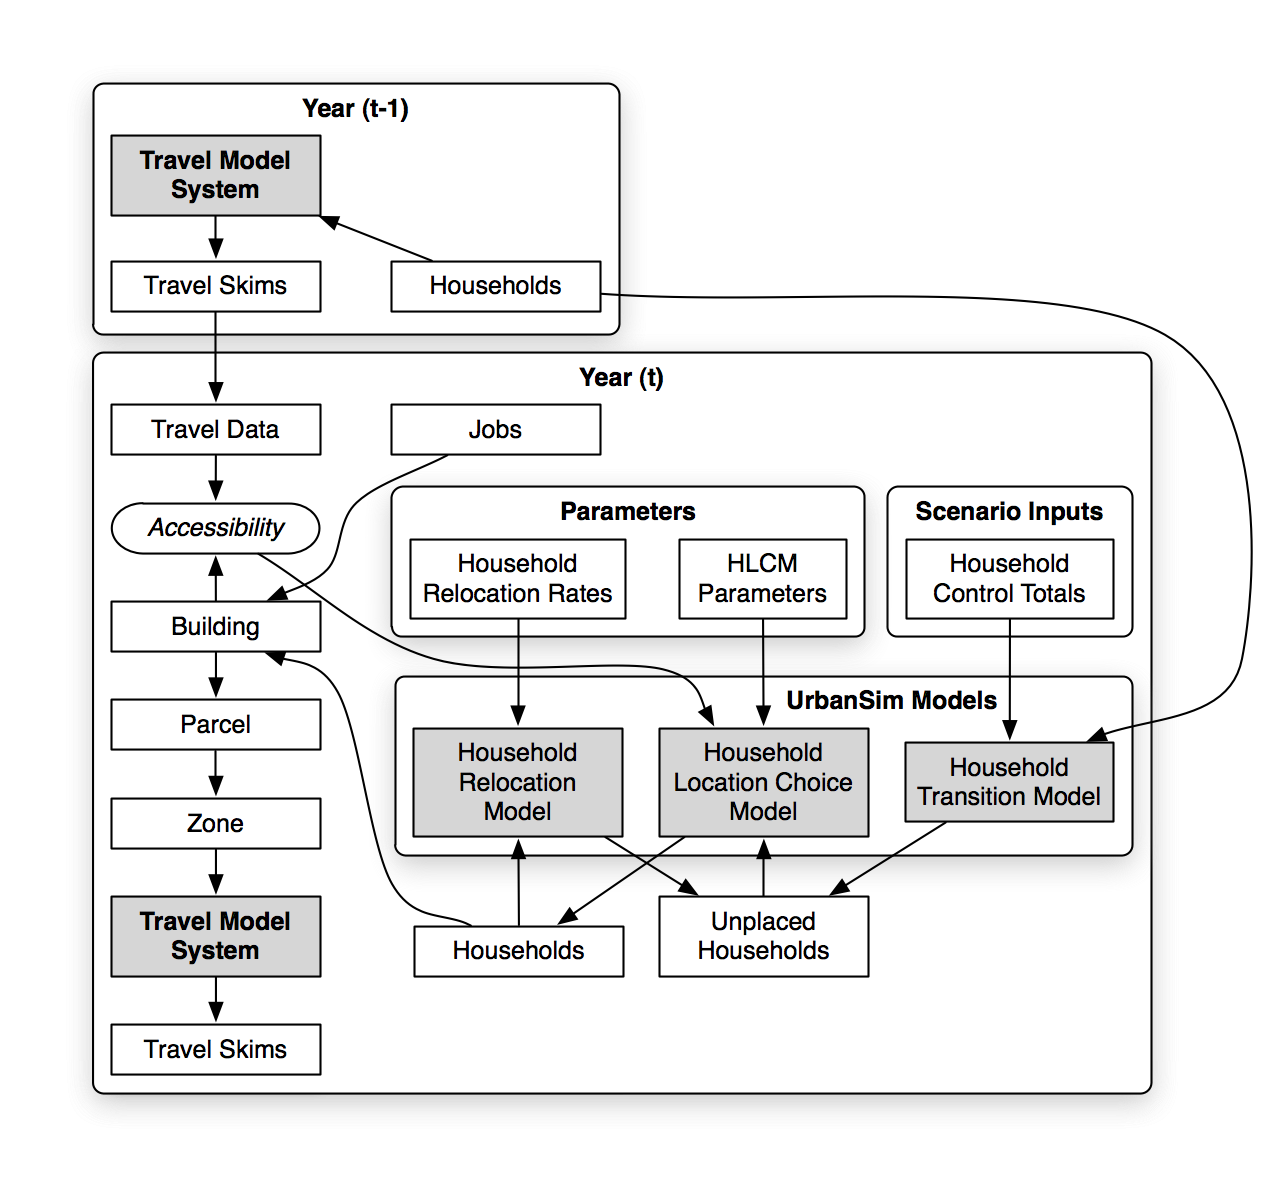
\includegraphics[width=\textwidth]{graphics/ParcelHouseholdModel.png}
    \caption{UrbanSim model flow: household focus}
    \label{fig:household-models}
\end{figure}

\begin{figure}[ht]
    \center
    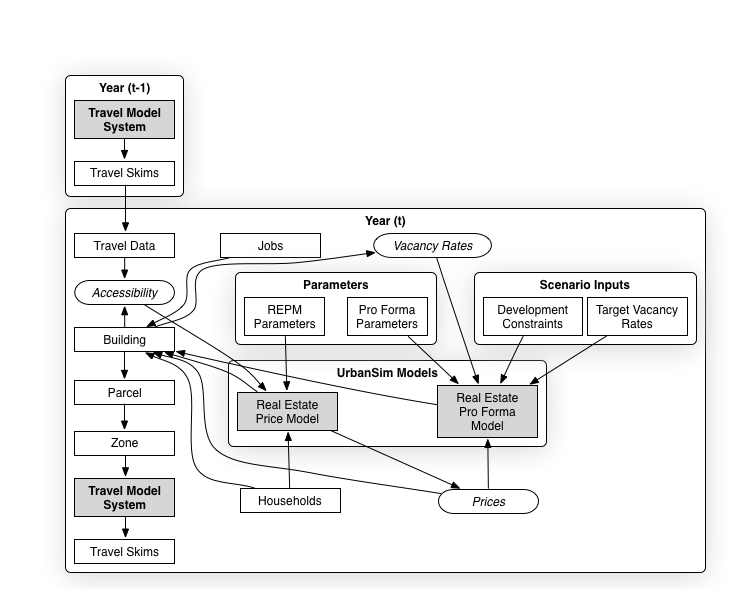
\includegraphics[width=\textwidth]{graphics/ParcelRealEstateModel.png}
    \caption{UrbanSim model flow: real estate focus}
    \label{fig:parcel-models}
\end{figure}

The model system contains a large number of components, so in order to make the illustrations clearer, there are three \enquote{views} of the system. In Figure \ref{fig:employment-models}, the focus is on the flow of information related to jobs. Figure \ref{fig:household-models} provides a household-centric view of the model system. Finally, Figure \ref{fig:parcel-models} provides a view with a focus on real estate.

UrbanSim predicts the evolution of these entities and their characteristics over time, using annual steps to predict the movement and location choices of businesses and households, the development activities of developers, and the impacts of governmental policies and infrastructure choices. The land use model is interfaced with a metropolitan travel model system to deal with the interactions of land use and transportation. Access to opportunities, such as employment or shopping, are measured by the travel impedance of accessing these opportunities via all available modes of travel.

%todo{In the sentence above does cost refer to travel time or monetary cost? If it refers to travel time then I would delete the word "cost" as the words "travel time" are already written}



\subsubsection{Discrete choice models}
\label{sec:discrete-choice}

UrbanSim makes extensive use of models of individual choice. A novel approach to modeling individual actions using discrete choice models emerged in the 1970s, with the pioneering work of McFadden on Random Utility Maximization theory
\citep{mcfadden-1974,mcfadden-1981}. This approach derives a model of the probability of choosing among a set of available alternatives based on the characteristics of the chooser and the attributes of the alternative, and proportional to the relative utility that the alternatives generate for the chooser.

Maximum likelihood and simulated maximum likelihood methods have been developed to estimate the parameters of these choice models from data on revealed or stated preferences, using a wide range of structural specifications \citep{train-book-2003}. Early application of these models were principally in the transportation field, but also included work on residential location choices \citep{quigley-eer-1976,lerman-trr-1977,mcfadden-1978}, and on residential mobility \citep{clark-vanlierop-1986}.

%\todo{From Emily: "households choosing among locations" makes the household seem like a decision maker}
%\todo{From Paul: Emily, households are actually considered the decision-making agent for residential location choices}
Let us begin with an example of a simple model of households choosing among alternative locations in the housing market, which we index by $i$. For each agent, we assume that each alternative $i$ has associated with it a utility $U_i$ that can be separated into a systematic part and a random part:

\begin{equation}
    \label{eq:utility}
    U_i = V_i + \epsilon_i
\end{equation}

where $V_i = \beta\cdot {x}_i$ is a linear-in-parameters function, $\beta$ is a vector of $k$ estimable coefficients,
$x_i$ is a vector of observed, exogenous, independent alternative-specific variables that may be interacted with the
characteristics of the agent making the choice, and $\epsilon_i$ is an unobserved random term. Assuming the unobserved term in \Cref{eq:utility} to be distributed with a Gumbel distribution leads to the widely used multinomial logit model \citep{mcfadden-1974,mcfadden-1981}:

\begin{equation}
    \label{eq:mnl}
    P_i = \frac{\mathrm{e}^{V_i}}{\sum_j \mathrm{e}^{V_j}}
\end{equation}

where $j$ is an index over all possible alternatives. The estimable coefficients of \Cref{eq:mnl}, $\beta$, are estimated with the method of maximum likelihood \citep{greene-2002}.

The denominator of the equation for the choice model has a particular significance as an evaluation measure. The log of this denominator is called the \emph{logsum}, or composite utility, and it summarizes the utility across all the alternatives. In the context of travel mode between origins and destinations, for example, it would summarize the utility (disutility) of travel, considering all the modes connecting the origins and destinations. It has theoretical appeal as an evaluation measure for this reason. In fact, the logsum from the mode choice model can be used as a measure of accessibility.

\begin{figure}[htbp]
    \center
    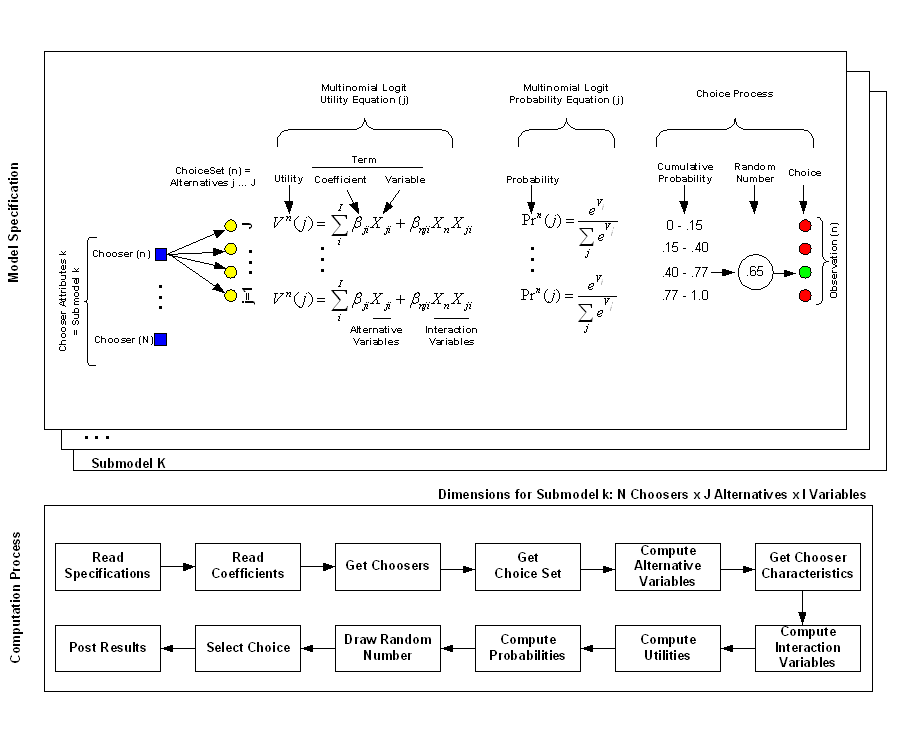
\includegraphics[width=\textwidth]
    {graphics/ChoiceProcess.png}
    \caption{Computation process in UrbanSim choice models}
    \label{fig:choiceprocess}
\end{figure}

Choice models are implemented in UrbanSim in a modular way, to allow flexible specification of models to reflect a wide variety of choice situations. Figure \ref{fig:choiceprocess} shows the process both in the form of the equations to be computed and from the perspective of the tasks implemented as methods in software.

For each model component within the UrbanSim model system, the choice process proceeds as shown in Figure \ref{fig:choiceprocess}. The first steps of the model read the relevant model specifications and data. Then a choice set is constructed for each chooser. Currently this is done using random sampling of alternatives, which has been shown to generate consistent, though not efficient, estimates of model parameters \citep{ben-akiva-lerman-1987}.

The choice step in this algorithm warrants further explanation. Choice models predict choice probabilities, not choices. In order to predict choices given the predicted probabilities, we require an algorithm to select a specific choice outcome. A tempting approach would be to select the alternative with the maximum probability, but unfortunately this strategy would have the effect of selecting only the dominant outcome, and less frequent alternatives would be completely eliminated. In a mode choice model, for illustration, the transit mode would disappear, since the probability of choosing an auto mode is almost always higher than that of choosing transit. Clearly this is not a realistic outcome.

In order to address this problem, the choice algorithm used for choice models uses a sampling approach. As illustrated in Figure \ref{fig:choiceprocess}, a choice outcome can be selected by sampling a random number from the uniform distribution in the range 0 to 1, and comparing this random draw to the cumulative probabilities of the alternatives. Whichever alternative the sampled random number falls within is the alternative that is selected as the \enquote{chosen} one. This algorithm has the property that it preserves in the distribution of choice outcomes a close approximation of the original probability distribution, especially as the sample size of choosers becomes larger.

\begin{figure}[htbp]
    \center
    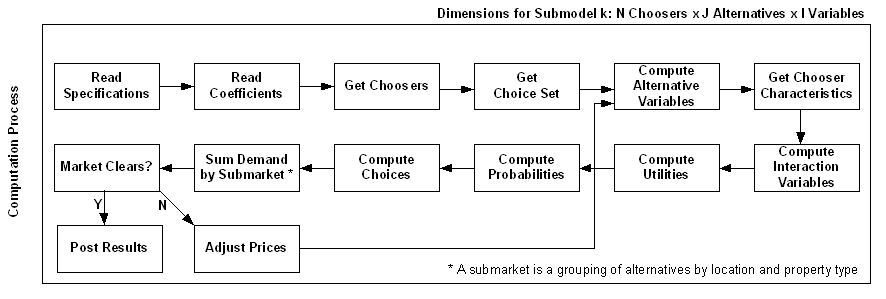
\includegraphics[width=\textwidth]
    {graphics/ChoiceProcessWithPriceAdjustment.png}
    \caption{Choice process with price adjustment in UrbanSim choice models}
    \label{fig:choiceprocesswithprice}
\end{figure}

We have also developed an alternative choice algorithm that enables the model to simulate short-term market clearing
processes. We compute the probability step of the location choice model, sum the probabilities at each submarket to compute
aggregate demand, and use this estimate of demand to compare to the available supply in the submarket. Prices are adjusted
iteratively and the relevant components of the location choice model are updated to reflect the influence of the adjusted
prices. This algorithm captures the feedback loop between excess demand for locations causing prices there
to increase, which in turn, dampens demand as the submarket becomes relatively more expensive than other submarkets that
are substitutes. This variant of the choice process is shown in Figure \ref{fig:choiceprocesswithprice}.

One other choice context is worth noting. In some situations, the availability of alternatives may be constrained. If the limit on availability is entirely predictable, such as a budget constraint eliminating expensive options, or a zero-car household being unable to use the drive-alone mode, this is straightforward to handle, by eliminating the alternatives from the choice set for those choosers. 

%In other situations, however, the solution is not so straightforward. In the case where alternatives may be unavailable because many other agents wish to choose them, the problem is that the alternative may be unavailable due to the endogenous congestion of alternatives. The effect of this is potentially significant, since it may cause parameters estimated in a choice model to confuse, or confound, the effects of preferences with the effects of constraints. Fortunately, an estimation method has been developed to account for this problem \citep{depalma-jue-2007}.

%\todo{From Emily: If it's worth explaining that an estimation method has been developed to account for this problem it is likely worth explaining what this solution method actually does?}


\subsection{Outputs}

As a microsimulation system, UrbanSim essentially produces the same outputs as it uses as inputs: tables of individual households and persons, jobs, parcels, buildings, with their attributes updated each simulation year if they have been modified by the model system.  New households, jobs and buildings are added or subtracted by the simulation, and households and jobs may relocate into or within the region.  By retaining this level of detail, UrbanSim is therefore able to generate summaries of the real estate data, demographics, or economic profile of any geographic aggregation requested by the user, such as census geographies, cities, counties, or other planning geographies.  Often traffic analysis zone summaries are used as inputs to the travel model system.  In this project our goal is to avoid losing information by aggregating the data to traffic zone when we connect UrbanSim to the travel demand model system.


\subsection{Calibration and validation}

UrbanSim is generally calibrated longitudinally, starting from an observed year in the past and running it to a later observed year, to compare predicted to observed data over time, and adjusting calibration coefficients iteratively to improve the fit of the model to the observed calibration targets at the calibration year.  Generally it is preferable to minimize the use of calibration constants since excessive use of calibration constants can 'handcuff' the model and make it insensitive to policy changes.

Some work has been done previously to extend this methodology to account for uncertainty using Bayesian Melding, to calibrate the model uncertainty and enable the computation of confidence intervals around its predictions, when running the model multiple times without fixing the random seed for the stochastic simulation \citep{sevcikova-tra-2009, sevcikova-tra-2011}.  